\chapter{Kokoonpano}

Toisena merkittävänä alueena ketterän ryhmän hallinnallisissa haasteissa on ryhmäkokoonpanoon liittyvät haasteet, kuten muutokset ryhmässä ja kokoonpanon suunnittelu. Suunnittelun merkitys korostuu kokoonpanoon liittyvissä tehtävissä, kuten vastuunjaossa. On kuitenkin huomioitavaa, että suunnittelun merkitys nykyaikaisessa ohjelmistokehityksessä on muuttunut luonteeltaan perinteisiin malleihin, kuten vesiputousmalliin, nähden. Toisaalta puutteet suunnittelussa on kuitenkin yksi yleisimmistä ketterää toteuttavan ryhmän hallinnallisten haasteiden lähteistä \cite{7872736}. Beck et al. \cite{beck2001agile} määrittävät yhtenä ketteristä periaatteista, että muutokseen reagointi on tärkeämpää kuin suunnitelmassa pysyminen.

Tutkimuksessaan de Melo et al. \cite{DEOMELO2013412} toteavat ketterän ryhmän hallinnan olevan suurin vaikuttava tekijä tuottavuuteen. Tutkimus kartoitti merkittävimmät tuottavuuteen vaikuttavat tekijät, minkä myötä ne rajattiin ketterän ryhmän sisäisiin ja ulkoisiin haasteisiin. Kuva \ref{fig:kokoonpanohaasteet} kokoaa ryhmän sisäiseen kokoonpanoon liittyvät haasteet ja niiden tekijät. Ryhmän sisäiset haasteet koostuvat suunnitteluvalinnoista sekä jäsenten vaihtuvuudesta ja niihin liittyvistä vaikutuksista, kun taas ulkoiset haasteet koostuvat useamman ryhmän välisestä yhteistoiminnasta. Seuraavissa alakappaleissa käsitellään ryhmäkokoonpanoon liittyviä sisäisiä haasteita. Kokoonpanoon liittyvä ulkoinen haaste käsiteltiin edellisessä kappaleessa osana koordinaatiota.


\begin{figure}[t]
\centering 
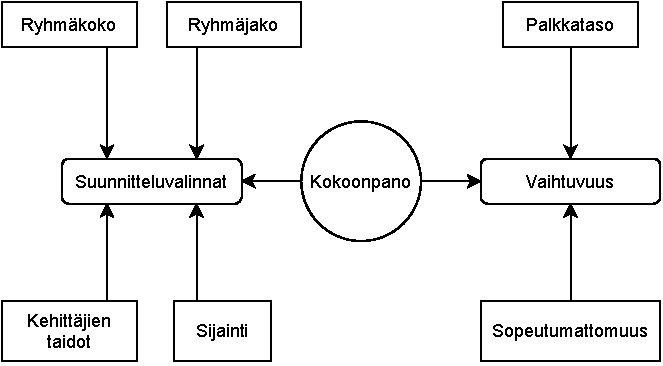
\includegraphics[width=0.9\textwidth]{template/figures/kokoonpanohaasteet.pdf}
\caption{Kaavio kokoonpanohaasteista ja niiden tekijöistä perustuen de Melo et al. \cite{DEOMELO2013412} ja Silva et al. \cite{SELLERISILVA201520} tutkimuksiin.\label{fig:kokoonpanohaasteet}}
\end{figure}


\section{Suunnitteluvalinnat}

Kuvan \ref{fig:kokoonpanohaasteet} mukaisesti ryhmän suunnitteluvalinnat koostuvat ryhmäkoosta, ryhmäläisten taidoista, ryhmäläisten keskinäisestä sijainnista sekä ryhmäläisten jaosta \cite{DEOMELO2013412}. De Melo et. al \cite{DEOMELO2013412} tutkimuksesta on tulkittavissa, että haasteita kokoonpanoon tuottaa tässä kontekstissa muun muassa seuraavanlaiset tilanteet. Kokoonpanossa, jossa valtaosa ryhmäläisistä olisi osa-aikaisia työntekijöitä keskinäinen keskittyminen projektiin voisi olla heikkoa perustuen tutkimuksen toteamukseen tapauksesta, jossa täyspäiväjäsenillä on parempi keskittyminen. Ryhmän monipuolisuus kokemusten ja taitojen osalta on todettu hyödylliseksi siten, että kokeneilla on laaja kokemuskirjo, kun taas vähemmän kokeneet ryhmäläiset ovat yleensä joustavampia. Kaiken kaikkiaan kokemustasojen erot parantavat ryhmän tuottavuutta. Ryhmäkokoon liittyen on todettu, että pienemmän ryhmän koordinaatio (erityisesti kommunikoinnin osalta), konfliktinhallinta, sitoutuminen sekä vastuuntunto ovat paremmalla tasolla kuin suuremmissa ryhmissä. Suuremman ryhmäkoon on todettu monimutkaistavan ryhmätyöskentelyä esimerkiksi siten, että useampi kehittäjä saattaa heikentyneen kommunikaation johdosta työskennellä tietämättään samojen asioiden parissa. Tästä aiheutuu ylimääräistä päällekkäistä työskentelyä, jonka myötä ryhmän tuottavuus heikentyy. Aiheeseen esitettiin myös vastaesimerkki, jossa kehittäjät eivät työskennelleet jonkin tehtävän parissa olettaessaan jonkun muun ryhmäläisen jo hoitavan sitä. Kommunikointihaasteiden lisäksi suuremman ryhmäkoon on todettu korreloivan suurempaan määrään konflikteja \cite{DEOMELO2013412, SELLERISILVA201520}. De Melo et al. \cite{DEOMELO2013412} toteavat ryhmän sijainnin vaikuttavan erityisesti vaatimusmäärittelyn ja suunnittelun toteutukseen siten, että paikallisessa ketterässä ryhmässä ne ovat huomattavasti helpompia. Paikallisen ryhmän kommunikointi sekä koheesio ovat myös parempia kuin esimerkiksi maantieteellisesti hajautetussa ryhmässä. Samassa sijainnista työskentelevien on todettu poistavan erilaisia sosiaalisia muureja ryhmäläisten väliltä mahdollistaen paremman kommunikaation. Työskentelysijainnin todettiin myös vaikuttavan tuottavuuteen perustuen sijainnin mielekkyyteen.

\section{Vaihtuvuus}

Ryhmäläisten vaihtuvuus on toinen ryhmän sisäistä haasteista. Vaihtuvuudeksi de Melo et al. \cite{DEOMELO2013412} määrittävät sekä aiemman kehittäjän lähtönä ryhmästä että uuden kehittäjän liittymisenä ryhmään. Vaihtuvuus aiheuttaa organisaatiolle monenlaisia kustannuksia, kuten irtisanoutumiseen, rekrytointiin sekä perehdyttämiseen liittyen. Lisäksi kehitysryhmä työskentelee vaihtuvuuden aikana astetta pienemmällä teholla johtuen joko pienemmästä määrästä kehittäjiä ryhmässä tai uuden ryhmäläisen perehdyttämisestä. Lisäksi uusien ryhmäläisten perehdyttäminen tehtävään on todettu haastavaksi \cite{SELLERISILVA201520} puhumattakaan siitä, että sopivien (tai hyvien) ryhmäläisten löytäminen on haastavaa \cite{GREGORY201692}. Tutkimuksessaan de Melo et al. \cite{DEOMELO2013412} määrittävät vaihtuvuuden tekijöiksi palkkatason sekä kehittäjän sopeutumattomuuden. Sopeutumattomuuden on arvioitu johtuvan muun muassa oma-aloitteisuuden ja sitoutumisen puutteesta, epäsopivasta personaallisuudesta muuhun ryhmään nähden sekä ryhmän sisäisistä erimielisyyksistä. Viimeisestä on tulkittavissa, että kommunikaatiohaasteet voivat aiheuttaa kokoonpanollisia haasteita. Epäsopivan persoonallisuuden omaavalla kehittäjällä tarkoitetaan tässä kontekstissa sellaista henkilöä, joka omalla olemuksellaan aiheuttaa toistuvasti konflikteja ryhmään.

Vaikka vaihtuvuus voi vaikuttaa negatiivisesti muun muassa lisäkustannuksien muodossa, sen on todettu vaikuttavan positiviisesti tilanteessa, jossa ryhmään liittyy uusi kehittäjä \cite{DEOMELO2013412}. Uudet ryhmäläiset saattavat tuoda uusia ideoita, ratkaisuja ja yleisesti ottaen energiaa ryhmään erityisesti tilanteessa, jossa ryhmän motivaatio on alhainen. Toisaalta vaihtuvuuden negatiivisia vaikutuksia on lukumäärällisesti enemmän ja ne voidaan jakaa pidentyneeksi tuotantoajaksi lyhyellä aikavälillä, oleellisen tiedon menettämisenä poistumisen yhteydessä sekä lisäkustannuksina. Pahimmassa tapauksessa projektin parissa ei työskentele yhtään alkuperäistä kehittäjää vaihtuvuuden seurauksena. Tällöin kriittistä tietoa projektiin liittyen on voinut kadota kokonaan.

De Melo et al. \cite{DEOMELO2013412} kiteyttävät ketterän ryhmän perustuvan yksilöihin ja ryhmätyöskentelyyn. Oikeilla menetelmillä toteutettuna kommunikaation ja yhteistyöskentelyn on todettu parantuvan. Tutkimus korostaa ketterien menetelmien prosessia tehostavia työskentelytapoja, kuten pariohjelmointia, päivittäistapaamisten ja yhteisistuntojen pitämistä. Kaiken kaikkiaan ketterien menetelmien oikeanlaisen ja tarpeeksi laajan toteutuksen on todettu vähentävän vaihtuvuuden riskiä. Toisaalta on syytä ottaa huomioon, että vaihtuvuus on varsin yleinen ilmiö. Vaihtuvuuteen liittyen ratkaisuksi on todettu tehokas tilanteeseen mukautuminen parhaalla mahdollisella keinolla.
